
% launchpad_mini
%-------------------------------------------------------------------------------
%
% \file        launchpad_mini.tex
% \library     Documents
% \author      Chris Ahlstrom
% \date        2021-01-24
% \update      2021-06-11
% \version     $Revision$
% \license     $XPC_GPL_LICENSE$
%
%     Provides a discussion of the MIDI input/output control
%     Launchpad Mini that Seq66 supports.
%
%-------------------------------------------------------------------------------

\section{Launchpad Mini}
\label{sec:launchpad_mini}

   This section discusses the configuration and usage of the
   \textsl{Novation Launchpad Mini} (we'll call it the "Mini")
   for control of patterns
   and for showing the status of \textsl{Seq66}.
   We will describe one of the 'ctrl' files provided with \textsl{Seq66},
   the setup of ports and connections 
   under ALSA and under JACK, and some related topics.

   A picture of the Mini appears at the end of this section.
   Supplemental information is documented in
   \texttt{contrib/notes/launchpad.txt} and
   \texttt{contrib/notes/launchpad-mini.ods} (a spreadsheet).

\subsection{Launchpad Mini Basics}
\label{subsec:launchpad_mini_basics}

   Let's start with a guide to Mini programming.
   Some of this information was adopted from the PDF file
   \texttt{launchpad-programmers-reference.pdf}.
   That document notes that a Mini
   message is 3 bytes, and is of type Note Off (80h), Note On (90h), or a
   controller change (B0h).  However, on our Mini, we do not receive Note Offs
   (in ALSA)... we receive Note Ons with velocity 0.

   The Mini has a top row of circular buttons numbered from 1 to 8.
   The next 8 rows start with 8 unlabeled square buttons on the left side
   with a circular button on the right, labelled with letters A through H.

   The top row's circular buttons (labeled "1" through "8")
   emit \texttt{0xB0 cc 0x7f} on press, and
   \texttt{0xB0 cc 0x00} on release, where:

   \begin{itemize}
      \item \textbf{0xB0}
         is a Control Change on channel 0.
      \item \textbf{cc}
         is a Control Change number, ranging from 0x68 (104 decimal)
         to 0x6f (111 decimal) which are in the range of
            \textsl{undefined} MIDI controllers.
   \end{itemize}

   The square buttons in the 8 x 8 matrix emit
   \texttt{0x90 nn 0x7f} on press, and \texttt{0x90 nn 0x0} on release, where:

   \begin{itemize}
      \item \textbf{0x90}
         is a Note On message on channel 0.
      \item \textbf{nn}
         is the hex value of the note, as shown by the two-digit hex values
            shown below.  The first "n" is the row number (from "0" to "7").
            The second "n" is the column (from "0" to "7", and "8" for the
            circular buttons.
   \end{itemize}

   The right columns's circular buttons (labeled "A" through "H"),
   emit the same kind of message, with note numbers of the form
   \texttt{n8}.

   There are two layouts available, \textbf{X-Y} and \textbf{Drum}.
   In \textsl{Seq66}, the drum layout is not used; see the
   file \texttt{contrib/notes/launchpad.txt}.

   X-Y Key Layout (mapping mode 1):

   \begin{verbatim}
           1     2     3     4     5     6     7     8 
    B0h: (68h) (69h) (6ah) (6bh) (6ch) (6dh) (6eh) (6fh)
    90h: [00h] [01h] [02h] [03h] [04h] [05h] [06h] [07h] (08h) A
         [10h] [11h] [12h] [13h] [14h] [15h] [16h] [17h] (18h) B
         [20h] [21h] [22h] [23h] [24h] [25h] [26h] [27h] (28h) C
         [30h] [31h] [32h] [33h] [34h] [35h] [36h] [37h] (38h) D
         [40h] [41h] [42h] [43h] [44h] [45h] [46h] [47h] (48h) E
         [50h] [51h] [52h] [53h] [54h] [55h] [56h] [57h] (58h) F
         [60h] [61h] [62h] [63h] [64h] [65h] [66h] [67h] (68h) G
         [70h] [71h] [72h] [73h] [74h] [75h] [76h] [77h] (78h) H
   \end{verbatim}

   The colors of the grid-buttons LED can be set via the command
   \texttt{90h key vel}, where:

   \begin{itemize}
      \item \textbf{0x90}
         is a Note On message on channel 0.
      \item \textbf{key} is a hex value given in the active of the
         two layouts shown above.
      \item \textbf{vel} is a bit mask of the form \texttt{00GGCKRR} where the
         bits have these meanings:
         \begin{itemize}
            \item \texttt{GG} for Green brightness.
            \item \texttt{C} to clear the LED setting of the other buffer.
               There are two buffers; see below for an explanation.
            \item \texttt{K} to copy the data to both buffers.
            \item \texttt{RR} for Red brightness.
         \end{itemize}
   \end{itemize}

   The Mini has two buffers 0 and 1 which contain two separate LED states. For
   example, in one buffer, all LEDs can be red, and in the other buffer, all LEDs
   can be green.  By default, buffer 0 is used for displaying and for writing.
   By alternating the buffers, the display can blink.

   The brightness values used for green and red range from 0 (off) to 3 (full
   brightness).  \textsl{Seq66} uses these values to provide red, green, yellow,
   and amber lighting.

   \begin{verbatim}
       Hex MSB  LSB
           00GG CKRR Color   Brightness Decimal Vel
       0Ch 0000 1100 Off     Off           12
       0Dh 0000 1101 Red     Low           13
       0Eh 0000 1110 Red     Medium        14
       0Fh 0000 1111 Red     Full          15
       1Ch 0001 1100 Green   Low           28
       1Dh 0001 1101 Amber   Low           29
       2Ch 0010 1100 Green   Medium        44
       2Eh 0010 1110 Amber   Medium        46
       3Ch 0011 1100 Green   Full          60
       3Eh 0011 1110 Yellow  Full          62
       3Fh 0011 1111 Amber   Full          63
   \end{verbatim}

   There are some other commands, not used, documented in
   \texttt{contrib/notes/launchpad.txt}.
   Also shown is a decimal version of the X-Y key layout.

   We use the square grid for toggling and showing pattern muting, and also for
   toggling mute groups.
   The top row of buttons are used for \textsl{Seq66}. We start with the basic
   controls, mapped to the top row of circular buttons (tentative):

   \begin{verbatim}
        Panic   Stop    Pause   Play    (free)    (free)  Set Dn   Set Up
   Dec   68h     69h     6ah     6bh     6ch       6dh     6eh      6fh
   Hex   104     105     106     107     108       109     110      111
   \end{verbatim}

   The Mini also supports power levels, but that feature is not used by
   \textsl{Seq66}.

\subsection{System Survey, ALSA}
\label{subsec:launchpad_mini_survey_alsa}

   Let's start with ALSA.  The following devices were discovered by running the
   commands \texttt{aconnect -lio} and \texttt{aplaymidi -l} and combining the
   information with the information shown on the
   \textbf{MIDI Clock} and \textbf{MIDI Input} tabs.

   \begin{verbatim}
   In  Out Port  Client name        Port name
            0:0  System             Timer
   [0]      0:1  System             Announce
   [1] [0] 14:0  Midi Through       Midi Through Port-0
   [2] [1] 28:0  Launchpad Mini     Launchpad Mini MIDI 1       (card 3)
   [3] [2] 32:0  E-MU XMidi1X1 Tab  E-MU XMidi1X1 Tab MIDI 1    (card 4)
   [4] [3] 36:0  nanoKEY2           nanoKEY2 MIDI 1             (card 5)
   [5] [4] 40:0  USB Midi           USB Midi MIDI 1             (card 6)
   \end{verbatim}

   Note the "Timer" device, which \textsl{Seq66} does not show, and the
   "Announce" device, which it does show (as disabled).  The device/port of
   interest is the \texttt{Launchpad Mini MIDI 1}, port 2 for input from
   the Mini, and port 1 for output to the Mini.

\subsection{Control Setup}
\label{subsec:launchpad_mini_control_setup}

   A couple of \textsl{Launchpad} control files are provided in the
   \texttt{/usr/share/seq66-0.93/data/linux} directory.
   Copy the \texttt{qseq66-lp-mini.ctrl} file to
   \texttt{\$HOME/.config/seq66}.
   Make sure to exit \textsl{Seq66} before the next steps.

   Open the \texttt{qseq66.rc} file.  Change

   \begin{verbatim}
      [midi-control-file]
      "qseq66.ctrl"
   \end{verbatim}

   to

   \begin{verbatim}
      [midi-control-file]
      "qseq66-lp-mini.ctrl"
   \end{verbatim}

   In \texttt{qseq66-lp-mini.ctrl}, first read through the file to get familiar
   with the format and purpose of this file.

\subsubsection{Input Control Setup}
\label{subsubsec:launchpad_mini_input_control_setup}

   We first want to use the Mini as a MIDI controller for
   the selection of loops, mute-groups, and various automation (user-interface)
   functions.
   In \texttt{qseq66-lp-mini.ctrl},
   the only change to make for input-control is
   to change \texttt{0xff} to the proper \textsl{input} port.  On our system,
   as noted above, that would be input port \texttt{[2]}.

   \begin{verbatim}
      [midi-control-settings]
      control-buss = 0xff     # change 0xff to 2
   \end{verbatim}

   Remember that \texttt{[midi-control-settings]} refers to controls
   \textsl{sent} to \textsl{Seq66} to control that application.
   Therefore, the control-buss is an input buss.
   Also remember that, in \textsl{ALSA}, \textsl{Seq66} detects and adds an
   "announce" buss as buss 0.  This extra buss is not seen via
   \texttt{arecordmidi -l}, but must be accounted for... it adds 1 to the
   number of each input buss.

   There are three sets of controls:  loops, mute-groups, and automation, as
   described in the following sections.

\paragraph{[loop-control]}
\label{paragraph:patterns_loop_control}

   In the \texttt{[loop-control]} section of \texttt{qseq66-lp-mini.ctrl},
   keystrokes are assigned, and only the "Toggle" (first)
   stanza of each MIDI control line
   is enabled, although there are definitions for the On and Off stanzas
   should one want to enable them.  Here are the first four lines, truncated.
   Note that they no longer include the "enabled" and "channel" columns.
   Instead, the event/status is checked to be non-zero in order to be enabled,
   and the channel is encoded in the event/status.

   \begin{verbatim}
      [loop-control]
       0 "1"  [ 0x90  0 1 127 ] [ 0x00  0 1 127 ] [ 0x00  0 1 127 ] ...
       1 "q"  [ 0x90 16 1 127 ] [ 0x00  0 1 127 ] [ 0x00 16 1 127 ] ...
       2 "a"  [ 0x90 32 1 127 ] [ 0x00 32 1 127 ] [ 0x00 32 1 127 ] ...
       3 "z"  [ 0x90 48 1 127 ] [ 0x00 48 1 127 ] [ 0x00 48 1 127 ] ...
       . . .
   \end{verbatim}

   The note values (0, 16, 32, 48) are in decimal. Why?
   Less to type, easier to understand.
   The whole \texttt{[loop-control]} section is 32 lines;
   only the top 4 rows of the Mini are shown here.
   Also note that, above, only the "Toggle" stanza is active.
   The "On" and "Off" stanzas use "0x00", which disables them, even
   if some data values are specified.

   If we want the loop armed only while the button is held, we would
   define something like:

   \begin{verbatim}
      [loop-control]
       0 "1"  [ 0x00  0 1 127 ] [ 0x90  0 1 127 ] [ 0x80  0 1 127 ] ...
       1 "q"  [ 0x00 16 1 127 ] [ 0x90  0 1 127 ] [ 0x80 16 1 127 ] ...
       2 "a"  [ 0x00 32 1 127 ] [ 0x90 32 1 127 ] [ 0x80 32 1 127 ] ...
       3 "z"  [ 0x00 48 1 127 ] [ 0x90 48 1 127 ] [ 0x80 48 1 127 ] ...
       . . .
   \end{verbatim}

   The pattern-number mapping for each Mini slot:

   \begin{verbatim}
        1     2     3     4     5     6     7     8 
      [  0 ] [  4 ] [  8 ] [ 12 ] [ 16 ] [ 20 ] [ 24 ] [ 28 ] A
      [  1 ] [  5 ] [  9 ] [ 13 ] [ 17 ] [ 21 ] [ 25 ] [ 29 ] B
      [  2 ] [  6 ] [ 10 ] [ 14 ] [ 18 ] [ 22 ] [ 26 ] [ 30 ] C
      [  3 ] [  7 ] [ 11 ] [ 15 ] [ 19 ] [ 23 ] [ 27 ] [ 31 ] D
   \end{verbatim}

   By pressing the appropriate button on the Mini, a pattern toggles between
   being armed and being muted.

\paragraph{[mute-group-control]}
\label{paragraph:patterns_mute_group_control}

   The mute-group controls are similar, except we didn't bother filling the On
   and Off stanzas at this time; they are all zeroes.

   \begin{verbatim}
      [mute-group-control]
       0 "!"  [ 0x90  64 1 127 ] ...
       1 "Q"  [ 0x90  80 1 127 ] ...
       2 "A"  [ 0x90  96 1 127 ] ...
       3 "Z"  [ 0x90 112 1 127 ] ...
   \end{verbatim}

   The mapping is the similar to loop-control, but offset by four rows.
   By pressing the appropriate button on the Mini, a mute-group toggles between
   being on (selected patterns armed) and off (all patterns muted).

\paragraph{[automation-control]}
\label{paragraph:patterns_automation_control}

   A large number of actions available from the user-interface can also be
   controlled by keystrokes or a MIDI device.  Here is a brief sample.  See the
   'ctrl' file itself for more information.

   \begin{verbatim}
      0 "'" [ 0x00 0 0 0 ] [ 0xb0 104 127 127 ] [ 0xb0 104 127 127 ] # BPM Up
      1 ";" [ 0x00 0 0 0 ] [ 0xb0 105 127 127 ] [ 0xb0 105 127 127 ] # BPM Dn
      2 "]" [ 0x00 0 0 0 ] [ 0xb0   0   0   0 ] [ 0xb0   0   0   0 ] # Set Up
      3 "[" [ 0x00 0 0 0 ] [ 0xb0   0   0   0 ] [ 0xb0   0   0   0 ] # Set Dn
   \end{verbatim}

   In \texttt{qseq66-lp-mini.ctrl}, all 64 square buttons are defined, which
   leaves the 16 circular buttons available for MIDI control. Only a few of those
   are defined so far.

\subsubsection{Output Control Setup}
\label{subsubsec:launchpad_mini_output_control_setup}

   Here, we want \textsl{Seq66} to send information to the Mini
   so that the lights on the Mini match the unmuted loops and 
   some of the \textsl{Seq66} controls.  Here are the changes to make to the
   output settings (while \textsl{Seq64} is \textsl{not} running).
   Change

   \begin{verbatim}
      [midi-control-out-settings]
      output-buss = 0xff
      midi-enabled = false
   \end{verbatim}

   to

   \begin{verbatim}
      [midi-control-out-settings]
      output-buss = 1
      midi-enabled = true
   \end{verbatim}

   If the device starts lighting up mysteriousy while playback is happen, make
   sure the music is not being played to the control device channe.
   Or, if your synth makes weird noises at startup/exit, make
   sure the output-buss setting is not pointing to your synth.
   (Been there, done that! \smiley{})

\paragraph{[midi-control-out]}
\label{paragraph:patterns_midi_control_out}

   The \texttt{[midi-control-out]} section provides a way to see the status of
   each pattern/loop in the Mini's grid.  Here are a few entries. As per the
   section above, 60 is green, 15 red, 62 is yellow, and 12 is off.

   \begin{verbatim}
       0 [ 0x90   0 60 ] [ 0x90   0 15] [ 0x90   0 62] [ 0x90   0 12]
       1 [ 0x90  16 60 ] [ 0x90  16 15] [ 0x90  16 62] [ 0x90  16 12]
       2 [ 0x90  32 60 ] [ 0x90  32 15] [ 0x90  32 62] [ 0x90  32 12]
       3 [ 0x90  48 60 ] [ 0x90  48 15] [ 0x90  48 62] [ 0x90  48 12]
   \end{verbatim}

   For the \texttt{qseq66-lp-mini.ctrl} file, only the upper 32 buttons and
   LEDS are used for this purpose, so there are 32 lines of data in this
   section.

   The four stanzas (numbers in square brackets) are:

   \begin{itemize}
      \item \textbf{Armed}.  This stanza is configured to show unmuted pattern
         slots as green.
      \item \textbf{Muted}.  This stanza is configured to show muted pattern
         slots as red.
      \item \textbf{Armed}.  This stanza is configured to show a queued pattern
         slots as yellow.
      \item \textbf{Armed}.  This stanza is configured to show an empty pattern
         slots as off (dark).
   \end{itemize}

\paragraph{[mute-control-out]}
\label{paragraph:patterns_mute_control_out}

   With the \texttt{qseq66-lp-mini.ctrl} file, the lower 32 buttons can be used
   to see which mute-group is selected (as well as to select a mute-group).
   The layout is pretty simple; here are the first four of the 32 lines:

   \begin{verbatim}
      1 [ 0x90  64 60 ] [ 0x90  64 15 ] [ 0x90  64 12 ]
      2 [ 0x90  80 60 ] [ 0x90  80 15 ] [ 0x90  80 12 ]
      3 [ 0x90  96 60 ] [ 0x90  96 15 ] [ 0x90  96 12 ]
      4 [ 0x90 112 60 ] [ 0x90 112 15 ] [ 0x90 112 12 ]
   \end{verbatim}

   The slots are numbered; all of the entries in the section are always
   enabled.  The first stanza indicates that the button the selected mute-group
   will be green.  The second stanza indicates that the unselected mute-group
   buttons will all be red, as long as they have mutes defined in them.  The
   third stanza indicates that the inactive (empty) mute-groups will be dark.

\paragraph{[automation-control-out]}
\label{paragraph:patterns_automation_control_out}

   This section allows for the following status to be shown in the top row of
   circular buttons:

   \begin{verbatim}
      1 [ 0xb0 104 60 ] [ 0xb0 104 0 ] # panic
      1 [ 0xb0 104 60 ] [ 0xb0 104 0 ] # play on/off
      1 [ 0xb0 104 15 ] [ 0xb0 104 0 ] # stop on/off
      1 [ 0xb0 104 62 ] [ 0xb0 104 0 ] # pause on/off
   \end{verbatim}

   Note that the play, stop, and pause statuses are all shown on the same
   button, as green, red, or yellow.  Some of these might still be in progress
   as you read this.

\subsection{Test Run, ALSA}
\label{subsubsec:launchpad_mini_test_run_alsa}

   Now that we're set up, start \textsl{Seq66}.

\begin{figure}[H]
   \centering 
   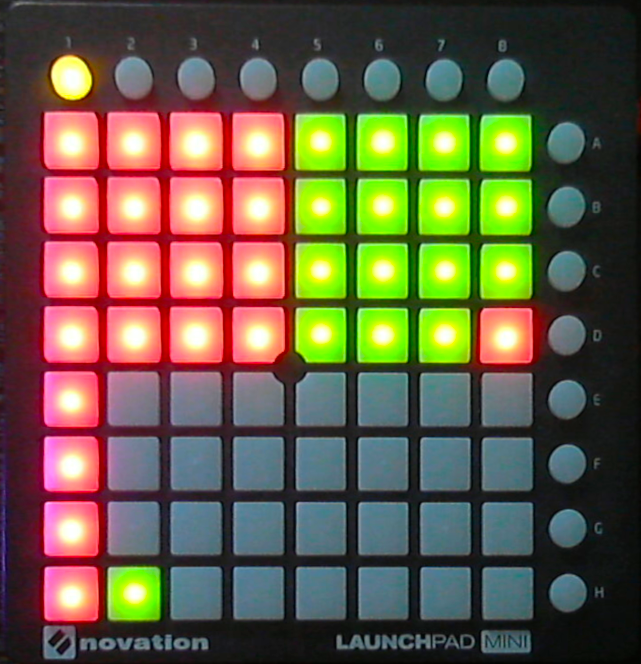
\includegraphics[scale=2.00]{configuration/ctrl/launchpad-mute-group-2.png}
   \caption{Launchpad Minu Running with Seq66}
   \label{fig:launchpad_mute_group_perspective}
\end{figure}

   This picture shows that playback is paused (yellow), that mute-group 7 is
   active, and that all the patterns in that mute-group are green, except for
   one that got muted accidentally while taking the pictre.

   If the \textbf{File / New} option is selected, all the patterns are turned
   off, but the four mute-group buttons at the bottom left remain, as the
   mute-groups are not erased.  (Bug or feature?)

   What's next?  First, add more controls and statuses to the configuration.
   Second, start working on a MIDI file to produce a light show!

\subsection{System Survey, JACK}
\label{subsec:launchpad_mini_survey_jack}

   Now let's see what we have to do in \textsl{JACK}.
   First peruse \sectionref{sec:jack}, to understand the basics about
   \textsl{JACK}, including the last section there that describes how to set up
   \textsl{ALSA}-to-\textsl{JACK} bridging.

   Run the following command, verify the ports in
   \textbf{Edit / Preferences / MIDI Clock} and \textbf{MIDI Input}, and then
   exit.

   \begin{verbatim}
      $ qseq66 --jack-midi
   \end{verbatim}

   In \texttt{qseq66.rc}, one will find this setting:

   \begin{verbatim}
      1     # with_jack_midi
   \end{verbatim}

   The MIDI inputs are shown, decorated with the "a2j" designation:

   \begin{verbatim}
   [midi-input]
   5   # number of input MIDI busses
   0 1 "[0] 0:0 seq66:a2j Midi Through [14] (capture): Midi Through Port-0"
   1 0 "[1] 0:1 a2j:Launchpad Mini [28] (capture): Launchpad Mini MIDI 1"
   2 0 "[2] 0:2 a2j:E-MU XMidi1X1 Tab [32] (capture): E-MU XMidi1X1 ..."
   3 0 "[3] 0:3 a2j:nanoKEY2 [36] (capture): nanoKEY2 MIDI 1"
   4 0 "[4] 0:4 a2j:USB Midi [40] (capture): USB Midi MIDI 1"
   \end{verbatim}

   This is very similar to the \textsl{ALSA} setup, except that there is no
   "announce" port in \textsl{JACK}.  The Mini's input buss has shifted from
   port 2 to port 1.  And, of course, the port names are a lot
   longer.  Similarly, for the MIDI outputs:

   \begin{verbatim}
   [midi-clock]
   5    # number of MIDI clocks (output busses)
   0 0  "[0] 0:0 seq66:a2j Midi Through [14] (playback): Midi Through. . ."
   1 0  "[1] 0:1 seq66:a2j Launchpad Mini [28] (playback): Launchpad. . ."
   2 0  "[2] 0:2 seq66:a2j E-MU XMidi1X1 Tab [32] (playback): E-MU . . ."
   3 0  "[3] 0:3 seq66:a2j nanoKEY2 [36] (playback): nanoKEY2 MIDI 1"
   4 0  "[4] 0:4 seq66:a2j USB Midi [40] (playback): USB Midi MIDI 1"
   \end{verbatim}

   We make sure that the correct \texttt{control-buss} and
   \texttt{output-buss} are set, and both have the setting
   \texttt{midi-enabled = true} in \texttt{qseq66-lp-mini.ctrl}.
   Then make sure that \texttt{qseq66.rc} has its
   \texttt{[midi-control-file]} set to:

   \begin{verbatim}
      "qseq66-lp-mini.ctrl"
   \end{verbatim}

   Run \texttt{qseq66} again, and make sure that the Mini's input and output
   ports are enabled. (Unfortunately, if one has to enable them, the
   application will need to be restarted.)
   The results should be just like
   \sectionref{subsubsec:launchpad_mini_test_run_alsa}.

%-------------------------------------------------------------------------------
% vim: ts=3 sw=3 et ft=tex
%-------------------------------------------------------------------------------
